\documentclass[10pt]{article}

\usepackage{adjustbox}
\usepackage{amsmath}
\usepackage[french, onelanguage]{algorithm2e}
\usepackage[utf8]{inputenc}
\usepackage[french]{babel}
\usepackage[T1]{fontenc}
\usepackage{geometry}
\usepackage{glossaries}
\usepackage{graphicx}
\usepackage[hidelinks]{hyperref}
\usepackage[utf8]{inputenc}
\usepackage{listings}
\usepackage{lstautogobble}
\usepackage{tabularx}
\usepackage{textcase}
\usepackage{tikz}
\usepackage{tocloft}
\usepackage{verbatim}
\usepackage{xcolor}
%\usepackage[pdf]{pstricks}
%\usepackage{auto-pst-pdf}
%\usepackage{uml}

\makeglossaries

\newacronym{gui}{GUI}{Graphical User Interface}
\newacronym{jdk}{JDK}{Java Development Kit}
\newacronym{ram}{RAM}{Random Access Memory}
\newacronym{json}{JSON}{JavaScript Oriented Notion}
\newacronym{ttmc}{TTMC}{Tu te mets combien?}

\usetikzlibrary{calc, shapes.multipart, chains, arrows}

\definecolor{RoyalBlue}{cmyk}{1, 0.50, 0, 0}

\lstset{language=C,
  keywordstyle=\color{RoyalBlue},
  basicstyle=\scriptsize\ttfamily,
  commentstyle=\ttfamily\itshape\color{darkgray},
  stringstyle=\ttfamily,
  breaklines=true,
  keepspaces=true,
  numbers=left,
  numbersep=5pt,
  showspaces=false,
  showstringspaces=false,
  showtabs=false,
  tabsize=4,
  autogobble=true
}

\geometry{
  a4paper,
  total={170mm,257mm},
  left=20mm,
  top=20mm,
}

\title{Tu te mets combien?}
\author{Giorgio Caculli LA196672, Guillaume Lambert LA198116, Tanguy Taminiau LA199566 \\ Groupe B05}
\date{\today}

\begin{document}
\maketitle

\newpage
\tableofcontents

\newpage
\section*{Introduction}
\label{sec:intro}
\addcontentsline{toc}{section}{\nameref{sec:intro}}
Dans le cadre du cours de ``Projets'' de l'UE 210, nous allons devoir créer un jeu similaire à ``\acrlong{ttmc}'' (\acrshort{ttmc}). L'objectif pédagogique de ce projet est de pousser l'élève a mieux appréhendé la librairie JavaFX vu au cours de 
POO (programmation orienté object). De plus la grande liberté accordé à ce projet consent et oblige l'élève à apprendre à se documenter et savoir faire des recherches.  L'objectif du projet est simple, créer un jeu sur le principe de TTMC (Tu Te 
mets Combien ?).  

\newpage
\section{Analyse de l'existant}
\subsection{Product backlog}
\noindent\adjustbox{max width=\textwidth}{
\begin{tabular}{| p{1cm} | p{16cm} |}
	\hline
	US-01 & En tant qu'utilisateur je voudrais savoir mon score.\\
	\hline
	US-02 & En tant qu'utilisateur je voudrais savoir si j'ai bien répondu.\\
	\hline
	US-03 & En tant qu'utilisateur je voudrais savoir si j'ai mal répondu.\\
	\hline
	US-04 & En tant qu'utilisateur je voudrais savoir quelle était la bonne réponse.\\
	\hline
	US-05 & En tant qu'utilisateur je voudrais savoir mettre mon jeu sur pause.\\
	\hline
	US-06 & En tant qu'utilisateur je voudrais savoir reprendre mon jeu où je l'avait laissé.\\
	\hline
	US-07 & En tant qu'utilisateur je voudrais savoir arrêter mon jeu à tout moment.\\
	\hline
	US-08 & En tant qu'utilisateur j'aimerais joué en multi joueur localement.\\
	\hline
	US-09 & En tant qu'administrateur je dois pouvoir ajouter une nouvelle carte au deck.\\
	\hline
	US-10 & En tant qu'administrateur je veux pouvoir supprimer une carte du deck.\\
	\hline
	US-11 & En tant qu'administrateur je veux pouvoir modifier une carte existante.\\
	\hline
	US-12 & En tant qu'utilisateur j'aimerais avoir une musique de fond.\\
	\hline
	US-13 & En tant qu'utilisateur j'aimerais pouvoir gérer le volume de la musique.\\
	\hline
	US-14 & En tant qu'utilisateur j'aimerais pouvoirs activer ou désactiver la musique de fond.\\
	\hline
	US-15 & En tant qu'utilisateur je voudrais pouvoir choisir mon propre pseudonyme.\\
	\hline
	US-16 & En tant qu'utilisateur je voudrais voir un plateau de jeu.\\
	\hline
	US-17 & En tant qu'utilisateur je voudrais avoir mon pion.\\
	\hline
	US-18 & En tant qu'utilisateur je voudrais savoir reconnaitre mon pion.\\
	\hline
	US-19 & En tant que joueur, je voudrais communiquer avec d'autre joueurs.\\
	\hline
	US-20 & En tant que joueur, j'aimerais jouer avec d'autre joueurs en ligne.\\
	\hline
	US-21 & En tant que joueur, j'aimerais rejoindre une partie en ligne.\\
	\hline
	US-22 & En tant que joueur, j'aimerais héberger une partie en ligne.\\
	\hline
\end{tabular}
}

\subsection{Les classes}

\subsubsection{Le modèle}

\subsubsection{La vue}

\subsubsection{Les exceptions}

\section{Description général de l'application}
Voici l'histoire d'un nain capable de courir vite et de voyager loin.\\
Dans son épopée formidable nous le suivrons une bière à la main.\\


\section{Product backlog}
\noindent\adjustbox{max width=\textwidth}{
\begin{tabular}{| p{1cm} | p{16cm} |}
	\hline
	US-01 & En tant qu'utilisateur je voudrais savoir mon score.\\
	\hline
	US-02 & En tant qu'utilisateur je voudrais savoir si j'ai bien répondu.\\
	\hline
	US-03 & En tant qu'utilisateur je voudrais savoir si j'ai mal répondu.\\
	\hline
	US-04 & En tant qu'utilisateur je voudrais savoir quelle était la bonne réponse.\\
	\hline
	US-05 & En tant qu'utilisateur je voudrais savoir mettre mon jeu sur pause.\\
	\hline
	US-06 & En tant qu'utilisateur je voudrais savoir reprendre mon jeu où je l'avait laissé.\\
	\hline
	US-07 & En tant qu'utilisateur je voudrais savoir arrêter mon jeu à tout moment.\\
	\hline
	US-08 & En tant qu'utilisateur j'aimerais joué en multi joueur localement.\\
	\hline
	US-09 & En tant qu'administrateur je dois pouvoir ajouter une nouvelle carte au deck.\\
	\hline
	US-10 & En tant qu'administrateur je veux pouvoir supprimer une carte du deck.\\
	\hline
	US-11 & En tant qu'administrateur je veux pouvoir modifier une carte existante.\\
	\hline
	US-12 & En tant qu'utilisateur j'aimerais avoir une musique de fond.\\
	\hline
	US-13 & En tant qu'utilisateur j'aimerais pouvoir gérer le volume de la musique.\\
	\hline
	US-14 & En tant qu'utilisateur j'aimerais pouvoirs activer ou désactiver la musique de fond.\\
	\hline
	US-15 & En tant qu'utilisateur je voudrais pouvoir choisir mon propre pséudonyme.\\
	\hline
	US-16 & Création d'un plateau de jeu.\\
	\hline
	US-17 & Implémentation du plateau de jeu.\\
	\hline
	US-18 & Creation des pions.\\
	\hline
	US-19 & Implémentation des pions de jeu et animation de mouvements des pions.\\
	\hline
	US-20 & Investiguer sur le multi joueur en ligne.\\
	\hline
	US-21 & Pion personnaliser.\\
	\hline
	US-22 & En tant que joueur, je voudrais communiquer avec d'autre joueur.\\
	\hline
	US-23 & En tant que joueur, j'aimerais jouer avec d'autre joueur en ligne.\\
	\hline
	US-24 & En tant que joueur, j'aimerais rejoindre une partie en ligne.\\
	\hline
	US-25 & En tant que joueur, j'aimerais héberger une partie en ligne.\\
	\hline
\end{tabular}
}


\section{Diagramme de classe}
%\umlDiagram[box=,sizeX=7cm, sizeY=7cm]{
%	\umlClass[]{Deck}
%	{}
%	{
%		\umlMethod[visibility]{add}{c \emph{BasicCard}}
%		\umlMethod[visibility]{remove}{c \emph{BasicCard}}
%		\umlMethod[visibility]{remove}{i \emph{int}}
%	}
%}
\begin{figure}[h]
	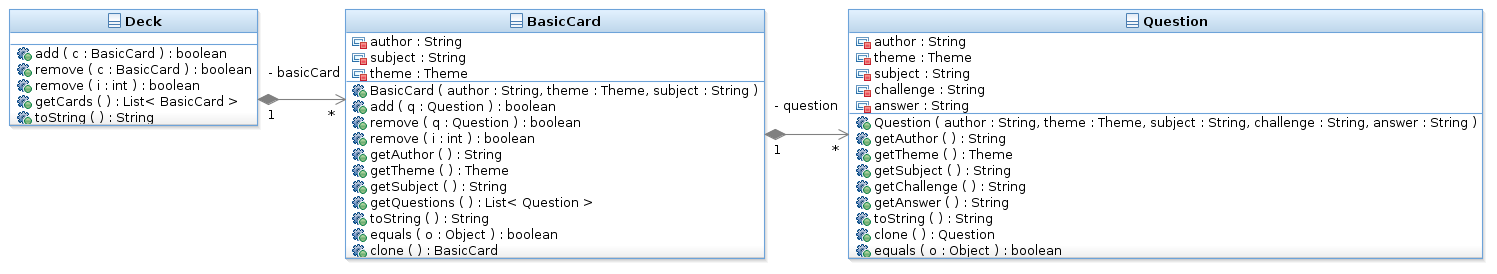
\includegraphics[width=\textwidth]{TTMC_Model_Diagram.png}
	\centering
\end{figure}


\section{Plan de sortie}
\begin{figure}[h]
	\centering
	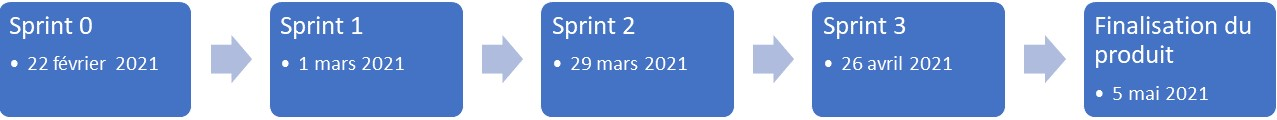
\includegraphics[width=\textwidth]{plan.jpg}
	\caption{Release plan}
	\label{fig:plan}
\end{figure}
\begin{itemize}
	\item Sprint 0 - Analyse et recherche.\\
	Cette première étape nous permettra de mettre en place le modèle du projet sur base de ce qui a été trouvé sur internet. Une fois compris les règles, il sera possible d'établir les fonctionnalités de base pour les composants principaux du programme ainsi que la mise en place des règles qui caractérisent chaque composant.
	\item Sprint 1 - Première démonstration en présence du Product Owner.\\
	Lors de la première démonstration, les différentes fonctionnalités seront testées. Les tests unitaires ne renverront aucun erreur et les différentes exceptions qui caractérisent chaque composant seront gérées.
	\item Sprint 2 - Deuxième démonstration du produit.\\
	Lors de la deuxième démonstration, un programme avec interface interactive sera mis en place. Ce prototype permettra d'interagir avec les différentes composantes et les manipuler librement.
	\item Sprint 3 - Troisième et dernière démonstration.\\
	Lors de la troisième démonstration, le programme aura une interface graphique basée sur JavaFX et toutes les interactions seront finalisées.
	\item Finalisation du produit - Présentation du produit final au client.\\
	Tous les bugs seront corrigés et toutes les interactions prévues seront fonctionnelles.
\end{itemize}

\newpage
\section{Prototype}
Dans cette section, nous vous présentons le prototype graphique.

\subsection{Menu principal}
Voici le menu principal, depuis celui-ci, il sera possible de jouer, de paramétrer le jeu, de quitter le jeu ou alors de gérer le jeu.
\begin{figure}[ht]
	\centering
	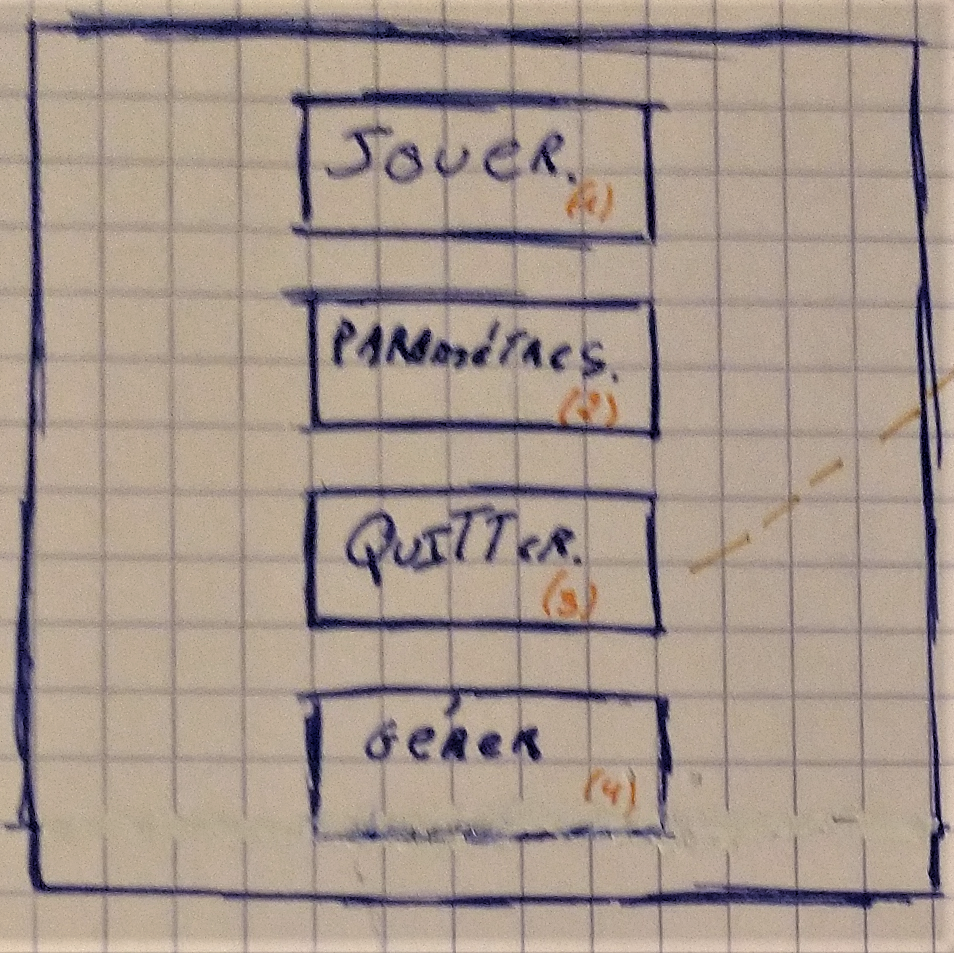
\includegraphics[scale=0.5]{menu_principal.png}
	\caption{menu principal}
	\label{interface menu}
\end{figure}

\newpage
\subsection{Menu joueur}
Le menu joueur sera un combo de label et de textfield, il sert à prendre des informations sur le nom des équipes. Il faut au minimum deux équipes ou joueurs.
\begin{figure}[ht]
	\centering
	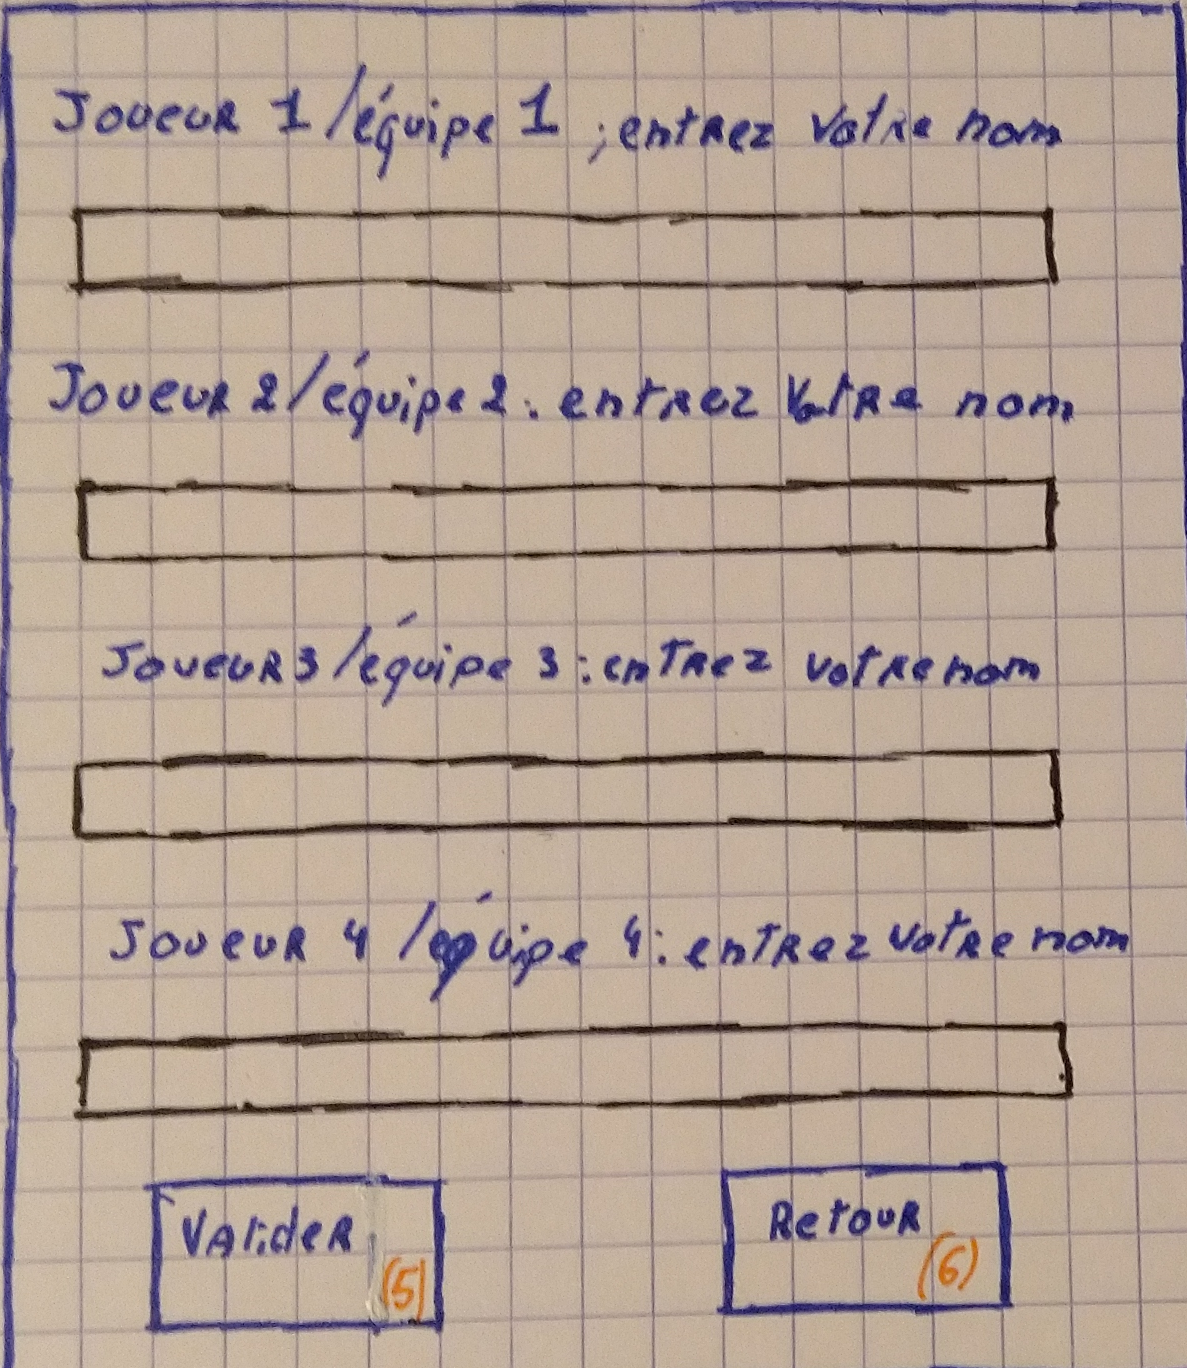
\includegraphics[scale=0.5]{menu_joueur.png}
	\caption{nom des joueurs ou équipe}
	\label{interface création d'équipe}
\end{figure} 

\newpage
\subsection{Fênetre erreur du nombre de joueurs}
Dans le cas où l'on n'entre pas suffisamment de joueur ou d'équipe, une alerte va notifier le joueur qu'il n'y a pas assez de joueur et ne peut donc pas jouer dans que cela n'est pas réglé.
\begin{figure}[ht]
	\centering
	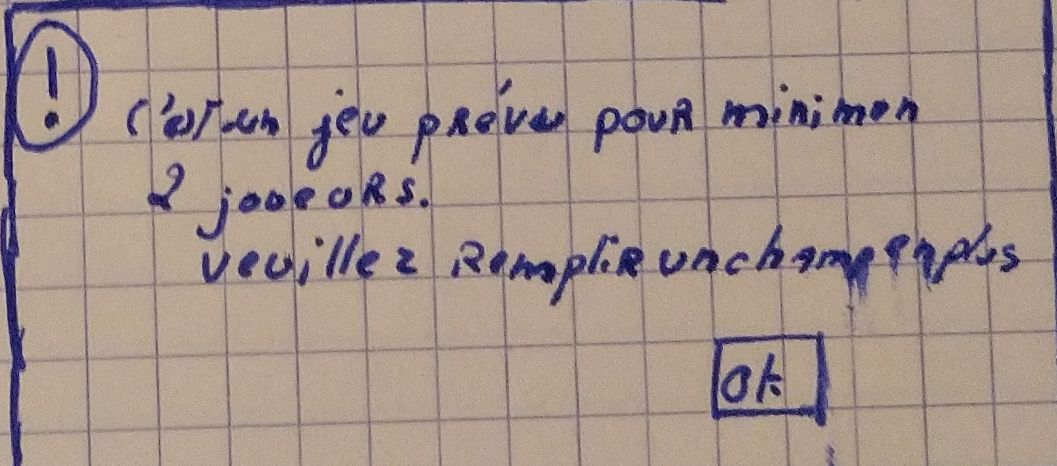
\includegraphics[scale=0.5]{fenetre_erreur_nb_joueur.png}
	\caption{alerte de non conformité du nombre de joueurs}
	\label{alerte du nombre de joueurs}
\end{figure}

\newpage
\subsection{Jeu}
Le UI sera composé d'un label avec le nom de l'équipe, un autre avec un des quatre thèmes, et un dernier avec le sujet de la question. Ensuite, il y a quatre boutons cliquable avec un numéro de un à quatre. Le numéro sur le bouton correspond 
à la difficulté de la question par ordre croissant.
\begin{figure}[ht]
	\centering
	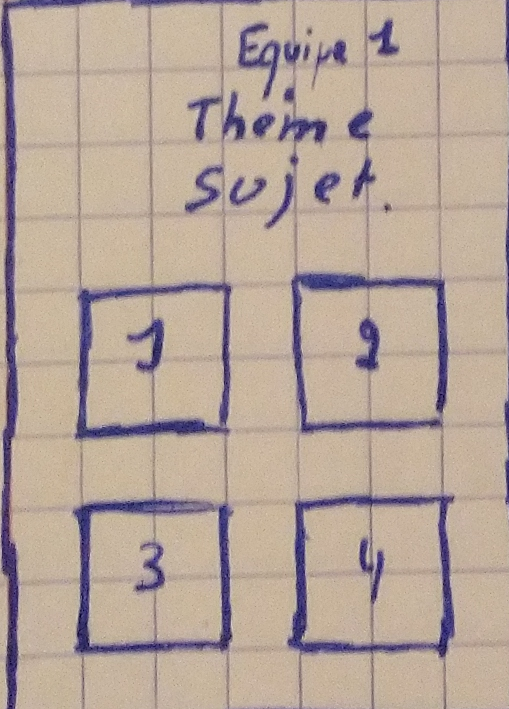
\includegraphics[scale=0.5]{jeux.png}
	\caption{choix de la difficulté de la question}
	\label{interface jeu}
\end{figure}

\newpage
\subsection{Fênetre quitter}
Il s'agit d'une fênetre permettant de vérifier si le joueur veux réellement quitter la partie. Cette fênetre est composer d'un label et de deux boutons permettant soit de quitter l'application, soit de retourner au menu principal.
\begin{figure}[ht]
	\centering
	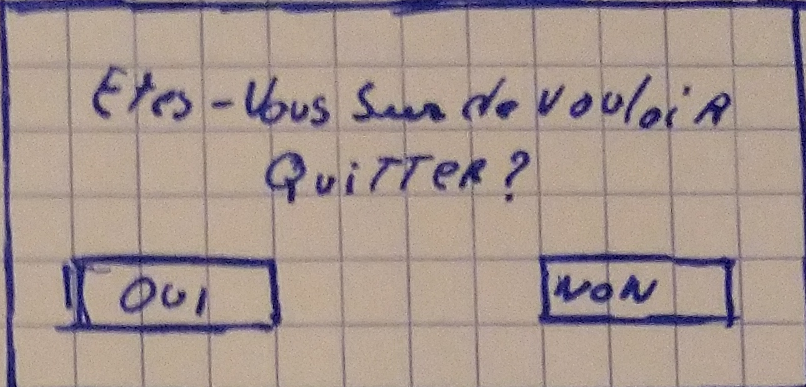
\includegraphics[scale=0.5]{fenetre_quitter.png}
	\caption{fêntre pour quitter le jeu}
	\label{fênetre pour quitter le jeu}
\end{figure} 


\newpage
\printglossary

\end{document}
